	% !TeX spellcheck = fr
	\section{Introduction}
	Les agents conversationnels connaissent un essor important  dans plusieurs domaines d'applications. Ces agents jouent différents rôles allant du rôle de tuteur pour enfant au compagnon pour les personnes âgées isolées.
	Dans le contexte de ces d'interactions,  l'agent et l'utilisateur humain  sont amenés à collaborer afin de satisfaire des tâches ou buts communs. Par exemple, un agent tuteur qui collabore avec un élève pour résoudre des exercices. Ils comparent leur connaissances respectives sur l'exercice à résoudre et discutent des solutions possibles. Une telle confrontation  permet d'offrir un enseignement personnalisé à l'élève. 
	
	En effet, la collaboration entre interlocuteurs pour la satisfaction de buts implique la confrontation des préférences et expertises de chacun des partis ce qui les conduit à négocier sur la manière de satisfaire le but en prenant en compte les préférences des deux partis. Ce type de négociation est appelée \emph{négociation collaborative.} A la différence de la négociation compétitive, la négociation collaborative fait l'hypothèse que chaque participant est motivé par le but de trouver le meilleur compromis satisfaisant les intérêts des deux participants au lieu de maximiser ses propres gains.
	
	Notre but est de modéliser un agent conversationnel capable d'avoir des négociations collaboratives crédibles avec un utilisateur humain.
	Pour ce faire, il est nécessaire de comprendre les comportements adoptés durant les négociations humains/humain. En effet,  Broekens \cite{broekens2010affective} présente la négociation comme un processus multidimensionnel qui implique une interaction sociale, des affects ainsi que des préférences et des opinions. La compréhension de l'aspect social est donc crucial pour l'étude du processus de négociation.
	De plus, la littérature en psychologie sociale a déjà démontré que la \emph{relation de pouvoir} a un effet direct sur les stratégies qu'utilisent les négociateurs.
	Il est par conséquent important pour un agent conversationnel qui négocie avec un utilisateur humain, de prendre en compte sa perception de la relation de pouvoir pour construire sa stratégie de négociation.
	
	Dans cette optique nous proposons dans ce papier, un agent conversationnel capable de mener une négociation collaborative avec un utilisateur humain. De plus, il est capable de déployer différentes stratégies de négociation en se basant sur la relation de pouvoir qu'il cherche à exprimer. Le plan de l'article se présente comme suit. La section 2 présente un état de l'art concis sur l'impact de la relation de pouvoir sur la négociation aussi bien en psychologie sociale qu'en informatique affective.  La section 3 présente les éléments de notre modèle de négociation collaborative. A partir d'un ensemble d'actes de dialogues et de préférences, nous proposons un modèle général de décision basé sur trois principes de négociation tirés de la psychologie sociale. Nous présentons en section 4 l'évaluation de notre modèle de négociation dans des interactions avec des utilisateurs humains qui montrent la pertinence des comportements implémentés. 
	
	\section{État de l'art}
		La notion de pouvoir social a été largement étudiée dans les domaines de la communication interpersonnelle et de la psychologie \cite{kecskes2013research}. Le pouvoir peut être défini comme la capacité à produire les effets voulus et à influencer le comportement de l'autre personne dans la conversation \cite {dunbar2005perceptions}. Dans le contexte de la communication et de la négociation, le pouvoir est une variable dyadique qui intervient au cours du dialogue.
		Les comportements liés au pouvoir peuvent contribuer positivement ou négativement au dialogue. Les contributions positives comprennent le maintien de la conversation et la prise de décisions rapides. Les contributions négatives incluent des comportements qui ont tendance à se focaliser sur soi et donc ne pas considérer le partenaire (\emph {e.g.} ne donnant pas l'occasion d'exprimer son opinion). Ce type de comportements peut être perçu comme blessant et offensant. Dans notre travail, nous nous concentrons sur des dialogues de négociation, dans lesquels plusieurs chercheurs ont déjà montré l'impact du pouvoir social \cite {de2004influence, burgoonnonverbal}.
	
		\subsection{Comportements de pouvoir dans les dialogues}
		\label{sec:domDialogue}
	
		Au cours d'un dialogue, le pouvoir peut se manifester à travers des comportements verbaux et non verbaux.
		Au niveau non verbal, un large éventail de comportements a été associé à la relation de pouvoir dont les mouvements kinesthésiques (expression faciale, mouvements corporels et gestes) et vocale (durée de la parole, intensité de la parole, contrôle de la voix et tonalité) \cite {burgoonnonverbal}. Sur la base de ce ces travaux, plusieurs agents conversationnels ont été développés avec la capacité d'exprimer un pouvoir social par le biais de comportements non verbaux, tels que le regard \cite {lance2008relation}, mouvements corporels \cite {mignault2003many} ou inclinaison de la tête  \cite {gebhard2014exploring} en relation avec la perception de pouvoir.
	
	
		Cependant, le pouvoir est également exprimé par des comportements verbaux. Un nombre considérable de recherches en sciences sociales et en communication ont documenté les effets du pouvoir sur les comportements utilisés par les négociateurs et donc sur les résultats de la négociation. De Dreu \cite {de1995impact} a démontré que les négociateurs avec un pouvoir élevé ont des aspirations plus grandes, ont plus d'exigences et concèdent moins. Galinsky \cite{galinsky2003power} affirme que le pouvoir renforce l'orientation des actions: les négociateurs de avec un pouvoir élevé contrôlent le flux de la négociation. En outre, la un pouvoir élevé augmente la direction de travaux avec des comportements axé sur la satisfaction des objectifs. Giebels \cite {giebels2000interdependence} montre que cela conduit les négociateurs avec un pouvoir élevé à se retrouver avec la part la plus grande du gâteau.
		
		En outre, le pouvoir affecte la manière dont les négociateurs collectent des informations sur leurs partenaires \cite {de2004influence}. Les négociateurs de faible pouvoir aspirent plus à développer une compréhension précise de leur partenaire et de ses comportements, chose qui les amènent à poser plus de questions  de \emph {diagnostic} que de questions \emph{directives}.
		
		Il a également été montré que les négociateurs de grande puissance sont égocentriques et ont tendance à ne pas prêter attention aux préférences des négociateurs avec un pouvoir plus faible \cite{fiske1993controlling, de1995impact}.
		
		Notre objectif est de développer un modèle de dialogue pour des agents virtuels qui prends en comptes ces propriétés liées au pouvoir social. Nous voulons rendre visibles \emph {les stratégies} déployées durant la négociation en fonction du pouvoir. Afin de mettre en œuvre ces différents comportements, nous avons identifié trois principes liés à la relation de pouvoir et leur impact sur la stratégie de négociation.
		
			\begin{enumerate}
				\item \textbf{Niveau d'exigence et de concessions:} Les négociateurs avec un pouvoir élevé affichent un niveau d'exigence plus important que les négociateurs avec un pouvoir plus faible. De plus, les exigences des négociateurs de faible pouvoir diminuent avec le temps il a tendance à faire des concessions plus importantes comparés a des négociateurs avec un pouvoir plus grand. \cite{de1995impact}
				
				\item \textbf{Soi Vs autrui:} Les négociateurs de faible pouvoir prennent en compte les préférences de l'autre dans la négociation, alors que les négociateurs avec un pouvoir plus grand sont égocentriques et ne s'intéressent qu'à satisfaire leurs propres préférences. \cite{fiske1993controlling,de1995impact}
				
				\item \textbf{Contrôle du flux de la négociation:}
				Les négociateurs avec un pouvoir élevé ont tendance à faire le premier pas \cite {magee2007power} et à prendre les devants dans la négociation. Les négociateurs de faible pouvoir visent à construire un modèle précis des préférences du partenaire de négociation, ce qui les amène à poser plus de questions afin de collecter des informations sur les préférences du partenaire au lieu de faire avancer la négociation (\emph{e.g}  faire des propositions)\cite{de2004influence}. 
				
			\end{enumerate}
	
			Dans le contexte de la négociation collaborative, nous devons combiner ces principes dans le but de trouver le meilleur compromis qui satisfasse les deux négociateurs.
			
		\subsection{Travaux similaires dans la littérature}	
		Seuls quelques chercheurs ont étudié l'expression du pouvoir dans le comportement verbal d'un agent conversationnel. \cite {bee2010bossy} a développé un agent qui exprime le pouvoir social à travers le regard et les caractéristiques linguistiques. Ils ont démontré que les traits de personnalité linguistiques influencent la perception du pouvoir. Cependant, ce travail ne considère pas comment le pouvoir affecte les stratégies de négociation dans le dialogue. Plus récemment, \cite{broekens2010affective, de2015humans} a étudié la confiance, l'expression des émotions comme de la colère et du bonheur comme dimensions de stratégies de négociations d'un agent virtuel. Cependant, cette recherche se concentre davantage sur l'aspect de la négociation que sur l'expression du pouvoir social. Dans notre travail, nous voulons étudier l'expression du pouvoir à travers la stratégie de dialogue, qui n'a pas été considérée par des travaux antérieurs.

		Dans un contexte différent, \cite {nazari2015opponent} a étudié comment la communication des préférences dans une négociation avec un humain peut avoir un impact sur les résultats de la négociation. Ils considèrent des situations dans lesquelles les négociateurs peuvent utiliser la tromperie pour obtenir un avantage déloyal et cacher leurs intentions. Nous ne considérons pas ce cas dans notre travail. Nos agents ne sont pas seulement collaboratifs, mais ils donnent également des informations correctes sur leurs préférences et ils n'essaient pas de cacher des informations. Des travaux antérieurs tels que \cite {swartout2006toward} ont montré que, même en négociation collaborative, il n'est pas toujours possible ni recommandé de donner des informations sur toutes les préférences.



	\section{Modèle de négociation basé sur la relation de pouvoir}
		
		Nous présentons dans cette section notre modèle de dialogue pour un agent virtuel dans le contexte de négociation collaborative. 
		Premièrement, nous présenterons le domaine de négociation à savoir la définition du sujet de conversation ainsi que les préférences sur ses valeurs. 
		Deuxièmement, nous présenterons notre algorithme de décision qui prend en compte les principes de comportements de pouvoirs (voir section 2.1) .
		
		\subsection{le domaine de la négociation}
			Le but de chaque processus de négociation est de trouver une \textbf{option} parmi un ensemble d'option $\mathcal{O}$. Le choix d'une option repose sur les critères qui caractérisent l'option.  Nous considérons l'ensemble $\mathcal{C}$ composé de $n$ critères, chacune disposant respectivement d'un domaine de valeurs  $C_1 \ldots C_n$. Nous pouvons donc représenté $\mathcal{O}$ comme le produit vectoriel de  $C_1\times\ldots\times C_n$ et chaque option $o \in \mathcal{O}$ comme un tuple $(v_1,\ldots,v_n)$ en faisant l'hypothèse que toutes les options d'un sujet donné sont toutes connues.
	
		
		Par exemple, pour un dialogue a propos des restaurants, les critères peuvent être le type de cuisine et le prix. Une option peut donc être représenté comme suit : $(Française, abordable)$
		
		\subsection{Le modèle des préférences}
			L'agent dispose d'un ensemble de préférences défini pour chaque critère $C_i$, formalisé comme un ordre partiel $ \prec_i$ sur les valeurs de ce critère. 
			Par exemple, si l'agent préfère la cuisine japonaise à la cuisine turque, on notera la relation de préférence $japonaise \prec_{cuisine} turque$. 
			
			A partir des relations de préférences, pour chaque critère $i\in \mathcal{C}$, pour chaque valeur $v\in C_i$, l'agent calcule la valeur de  \emph{satisfaction} $sat_{self}(v \prec_i)$ pour cette valeur comme le nombre de valeurs qu'il préfère moins dans l'ordre partiel des préférences $\prec_i$ normalisé entre $[0,1]$:
			
					\begin{equation}
					sat_{self}(v, \prec_i) =	1 - \left( \frac{|\{v' : v' \neq v \  \wedge \ (v \prec_i v')\}| }{( |C_i| - 1 )}\right)
					\end{equation}
					
			La notion de satisfaction est généralisée aux options $o= (v_1, \ldots, v_n)\in \mathcal{O}$ comme une moyenne: 
				\begin{equation}
				sat_{self}(o, \prec) = \frac{\sum_{i=1}^{n} sat_{self}(v_i, \prec_i) }{n}
				%\vspace{-1.5em} 
				\end{equation}
				
			La notion de satisfaction est utilisée tout au long du processus décisionnel de la négociation. Elle représente la tendance d'accepter ou rejeter une proposition, aussi bien que la valeur à proposer. Plus la valeur de satisfaction approxime 1, plus tôt elle sera sélectionnée au cours de la négociation.
			 
			 
		\subsection{Le modèle de dialogue}
		\label {sec:com}
		Les négociateurs communiquent pendant la négociation en utilisant des \emph {actes de dialogue}. Chaque acte de dialogue possède un ensemble spécifique d'arguments et est associé à une expression en langage naturel (NL). Nous utilisons cinq types d'actes de dialogues, basés sur le travail de Sidner \cite {sidner1994artificial} et deux actes supplémentaires pour conclure la négociation. la table \ref {table:utt} résume les différents actes de dialogues  génériques. 
		
		Comme les expressions dépendent du domaine d'application, seule la génération NL de ces énoncés doit être spécialisée. Dans cet article, nous illustrerons ce modèle par une négociation collaborative sur les restaurants. La valeur / $ v $ / dans la table \ref {table:utt} fait référence à ce format  en NL pour exprimer une valeur.
		
		Chaque type d'acte prend comme paramètre soit une valeur de critère $v \in C_i$, une option $o \in \mathcal{O}$, ou un critère $i \in \mathcal{C}$. 
		Nous distinguons trois groupes d'actes. Premièrement, les actes informatifs (\textit{AskValue/AskCriterion} et \textit{StateValue}) qui sont utilisés pour échanger des informations sur les préférences des interlocuteurs.  Nous avons remarqué que dans les interactions humain-humain, les interlocuteurs expriment implicitement leur préférences en spécifiant ce qu'ils aiment ou pas ( \emph{e.x.}\textit{I like Chinese more than French}) au lieu de faire une comparaison binaire
		
		Deuxièmement, les actes de négociation (\textit{Propose}, \textit{Accept} and \textit{Reject}) permettent à l'agent de mener la négociation soit en ouvrant des propositions ou en accepter/ rejeter une. Une proposition peut concerner soit une valeur de critère (``Let's go to a Chinese restaurant'') ou bien une option (``Let's go to \emph{Chez Francis} restaurant'').
		
		Troisièmement, les actes de fermeture de négociation (\textit{NegotiationSuccess} or \textit{NegotiationFailure}) sont utilisés pour clore un dialogue. 
		Des exemples de dialogues utilisant ces actes sont présentés dans la section \ref{sec:eval}.
		
		Le processus de décision pour la sélection du prochain acte de dialogue est basé sur nos trois principes qui sont décrits dans la section \ref{sec:decision}. Pour effectuer cette sélection, l'agent garde une trace de toutes les déclarations et propositions faites au cours du dialogue. Pour chaque critère $ i \in \mathcal{C} $, nous construisons l'ensemble $ S_i \subseteq C_i $  les valeurs préférences que l'agent a communiqué pour ce critère. Cela évite les reformulations d'informations précédentes. Nous construisons aussi les ensembles $ A_i \subseteq C_i $ et $ U_i \subseteq C_i $ des valeurs qui ont été déclarées comme aimées ou détestées par les expressions \emph {StateValue} de l'interlocuteur. Nous supposons que $ A_i \cap U_i = \emptyset $.
		
		Nous maintenons aussi les ensembles $ P_i \subseteq C_i $, $ T_i \subseteq C_i $ et $ R_i \subseteq C_i $ de toutes les valeurs proposées, acceptées et rejetées pour chaque critère. Ceux-ci seront utilisés pour faire des propositions pertinentes. De même, nous considérons $ P \subseteq \mathcal {O} $, $ T \subseteq \mathcal {O} $ et $ R \subseteq \mathcal {O} $ les ensembles de toutes les options proposées, acceptées et rejetées durant le dialogue.
			\begin{table}[t]
				{%\scriptsize
					\begin{tabular} {|p{2cm}|p{3.5cm}|p{2.5cm}|}
						\hline
						\textbf{Utterance type}  &\textbf{ NL generation} & \textbf{Postcondition}\\
						\hline
						StateValue(v) &  I (don't) like /$v$/. & Speaker : $v \in S_i$ \newline Hearer:  \newline $v\in A_i$ is likable, $v\in U_i$ otherwise \\
						\hline
						AskValue(v)& Do you like /$v$/ ? & \multirow{2}{*}{} \\
						
						AskCriterion(i) &  What kind of /$i$/ do you like ? & \\
						\hline
						ProposeOption(o)  & Let's go to /$o$/. & $o \in P$\\
						
						ProposeValue(v) & Let's go to a /$v$/. & $v \in P_i$\\
						\hline
						AcceptOption(o)& Okay, let's go to /$o$/.& $o \in T$ \\
						
						AcceptValue(v) & Okay, let's go to a /$v$/.& $v \in T_i$ \\
						\hline
						RejectOption(o) & I'd rather choose  something else. & $o \in R$\\
						
						RejectValue(v) &  I'd rather choose  something else. & $v \in R_i$ \\
						\hline
						Negotiation Success &  We reached an agreement. & \multirow{2}{*}{}\\
						\cline{1-2}
						Negotiation Failure &  Sorry, but I no longer want to discuss this. & \\
						\hline
						% Counter Propose & $(r,p)\in C_i^2 \vee (r,p) \in \mathcal{O}^2 $ & I don't want to go to $r$. Let's rather go to $p$ \\
						% \hline 
						% RejectState & $x \in \mathcal{O} \vee x\in C_i$ &  I don't like /$x$/, let's choose something else. \\
						% \hline
						% AcceptPropose & $o \in \mathcal{O}$ & Okay. Let's go to /$o$/.\\
						% \hline
					\end{tabular}
				}
				\caption{\label{table:utt}Liste des actes de dialogue.}
			\end{table}
			
			
			\subsection{Satisfaction de l'autre}
				En utilisant les ensemble $A_i$ et $U_i$ qui représentent les goûts de l'interlocuteur, l'agent peut calculer la satisfaction d'une valeur $v\in C_i$ pour l'interlocuteur en utilisant la formule suivante: 
				
				Notez que certaines valeurs peuvent rester inconnues: dans une négociation collaborative, ces valeurs peuvent être considérées comme potentiellement satisfaisantes. Par conséquent, nous leur donnons une valeur arbitraire fixée à 0.5.
					\begin{equation}
					sat_{other}(v)= \left\{\begin{array}{ll}
					1	 & \mathrm{if\ }  c \in A_i\\
					0    & \mathrm{if\ }c \in U_i\\
					0.5	 & \mathrm{otherwise}
					\end{array}\right.
					\end{equation}
				Cette formule est généralisable aux options $o=(v_1,\ldots,v_n) \in O$:
				
				\begin{equation}
				sat_{other}(o, A, U) = \frac{ \sum_{i}^{n} sat_{other}(v_i, A_i, U_i) } {n}
				\end{equation}
			
			La satisfaction représente l'attente qu'a un agent a propos du comportement de son interlocuteur pour soit accepter ou rejeter une proposition. Il sera utilisé pour sélectionner la proposition la plus tolérable à faire dans la négociation. Le concept de tolérable est présenté dans le section suivante.	
			
			
			\subsection{Processus de décision basé sur le pouvoir dans la négociation}
			\label{sec:decision}
			Dans la section \ref{sec:domDialogue}, nous avons identifié trois principes liés à la relation de pouvoir qui affecte les stratégies et comportements des négociateurs. Dans cette section, nous présentons la théorie computationnelle implémentant chaque principe.
			
			Nous désignons la croyance de l'agent de sa puissance $ pow \in [0, 1] $. C'est une constante pour un agent donné dans une interaction donnée.
			
			\subsubsection {Niveau d'exigences et de concession}
			
			En négociation collaborative, les deux participants réduisent leur niveau d'exigences au fil du temps dans le but de parvenir à un accord. Cependant, selon notre premier principe, le niveau d'exigence devrait être plus haut pour les agents avec un pouvoir élevé et les concessions devraient être plus importantes pour les agents avec un pouvoir faible. Pour modéliser ce comportement, nous utilisons une \emph {courbe de concession} illustrée dans la figure \ref {fig:conc}.
			
			Soit $ self (pow, t) $ une valeur variant dans le temps, suivant la courbe de concession:
				\begin{equation}
				self(pow, t) = \left\{\begin{array}{ll}
				pow & \mathrm{if\ } (t \leq \tau)\\
				max(0, pow - (\frac{\delta}{pow} \cdot (t - \tau))) & \mathrm{otherwise}
				\end{array}\right.
				\end{equation}
	
				\begin{floatingfigure}[r]{1.8in}
					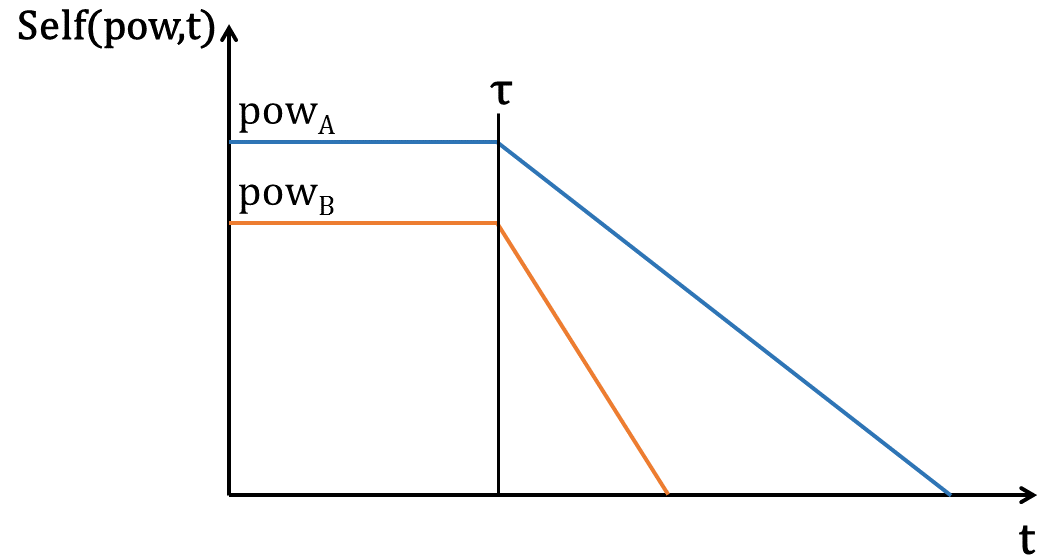
\includegraphics[width=1.8in]{graphs/sv3.png}
					\caption{\label{fig:conc}Courbe de concession}
				\end{floatingfigure} 
				
			Où est $ t \geq 0 $ est le nombre de propositions ouvertes ou rejetées, $ \tau> 0 $ est le nombre minimum de propositions avant le début de la concession et $ \delta> 0 $ est un paramètre de calcul pour la courbe de concession.
		
		La valeur $ self (pow, t) $ représente le poids qu'un agent donne à son autosatisfaction par rapport à la satisfaction de son partenaire. Plus le pouvoir de l'agent est élevé, plus ses exigences sont élevées. De plus, la courbe diminue plus vite pour les agents avec un pouvoir faible.
		
		Ces comportements d'exigence et de concession sont implémentés pour calculer \textit{l'acceptabilité} d'une valeur. Basé sur la valeur de satisfaction, l'agent peut décider de soit accepter ou rejeter une valeur.
		
		L'acceptabilité d'une valeur $ v \in C_i $ est définie comme une fonction booléenne:	
		
		\begin{equation}
	%	\vspace{-.5em} 
		acc(pow,v, t) = sat_{self}(v, \prec_i) \geq  (\beta \cdot self(pow,t))
		\end{equation}	
		où $ \beta> 0 $ est un paramètre de la théorie qui définit le poids donné au niveau d'exigence.
		
		Cette fonction est généralisable à toutes les options,  $o \in O$: $acc(pow,o, t) = sat_{self}(o, \prec) \geq  (\beta \cdot self(pow,t))$.
		
		\subsection{Soi Vs autrui}
	
		Selon notre second principe, les négociateurs avec un pouvoir élevé donnent plus de poids à leur propre satisfaction. Pour implémenter ce principe dans le contexte d'une négociation collaborative, nous calculons dans quelle mesure une proposition donnée est \textit{tolérable} en considérant la satisfaction de l'agent et de son partenaire.
		
		Pour un critère $i \in \mathcal{C}$, nous considérons le sous ensemble $V_i\subseteq C_i$ des valeurs acceptables pour l'agent: 
			\begin{equation}
			V_i(pow,t) = \{ v\in C_i : acc(pow,v,t) \}
		%	\vspace{-0.5em}
			\end{equation}
		
		
		Nous calculons la tolérabilité d'une valeur donnée $ v \in V_i (pow, t) $ en équilibrant entre les préférences de l'agent et les goûts de son partenaire. Nous supposons que l'agent donne un poids à la satisfaction de son partenaire qui est complémentaire à son auto-satisfaction:
			\begin{equation}
			\begin{split}
			tol(v, t, \prec_i, A_i, U_i, pow) & = self(pow, t)  \cdot sat_{self}(v, \prec_i) \\
			& +  (1 - self(pow, t)) \cdot sat_{other}(v, A_i, U_i)
			\end{split} 
			\end{equation}
		
		
		Nous généralisons cette fonction aux options $o=(v_1,\ldots,v_n) \in O$:
		
		\begin{equation}
		tol(o, t, \prec, A, U, pow) = \frac{ \sum_{i}^{n} tol(v_i, t, \prec_i, A_i, U_i, pow) } {n}
		\end{equation}
		
		\noindent
		L'agent propose toujours la valeur la plus tolérable dans le sous ensemble $V_i$:
		\begin{equation}
		propose(V_i, \prec_i,pow) =  \operatorname*{arg\,max}_{v \in V_i} ( tol(v))
		\end{equation}
		
		
			\subsubsection*{Résumé des paramètres d'implémentation }
			\begin{itemize}[noitemsep]
				
				\item $\pi \in $[0,1] : La limite entre le comportement dominant et soumis. Elle est utilisée dans le processus de choix d'acte de dialogue
				\item $\beta$:  une valeur qui représente le score minimum qu'une valeur doit obtenir pour être positivement satisfiable aux préférences de l'agent dans la négociation. Notons que $\beta = const \times self(dom,t)$.
				\item $\tau > 0$ : le nombre minimal de propositions ouvertes ou rejetées avant le début des concessions
				\item $\delta > 0$ : paramètre de la courbe de concession.
				\item $\alpha> 0$: Le nombre maximum d'actes informatifs successifs.
			\end{itemize}
		
		\subsubsection {Contrôle de la négociation}
		Le troisième principe relate que les négociateurs avec un pouvoir élevé ont tendance à mener la négociation. Nous avons implémenté ce principe à travers le choix des actes de dialogue présentés dans table \ref {table:uttChoice}.
		
		Nous avons défini un seuil $ \pi $ pour diviser le spectre de pouvoir en deux.
		
		En fonction du pouvoir, de l'acte de dialogue précédent $ u ^ {- 1} $ et de l'état du dialogue actuel, l'agent sélectionne le premier acte dans la table \ref {table:uttChoice} pour lequel la condition est satisfaite. 
		Par exemple, un agent avec un pouvoir élevé arrêtera la négociation dès que toutes les options restantes seront inacceptables (ligne 2). Un agent avec un pouvoir faible rejettera et indiquera une préférence, afin d'expliquer pourquoi la proposition n'est pas acceptable (ligne 14). S'il n'y a pas de proposition ouverte, l'agent avec un pouvoir faible demandera de nouvelles informations (ligne 18 -19).
		
		Dans notre modèle, un agent peut exprimer plus d'un acte de dialogue durant son tour de parole qui est représenté avec le signe "+" dans la table \ref {table:uttChoice}.
		
		Notez qu'un agent avec un pouvoir élevé se concentrera sur le maintien de la négociation en choisissant  des \emph{actes de négociation} (ProposeValue / ProposeOption, RejectValue / RejectOption, AcceptValue / AcceptOption) comme présenté dans les lignes (4 à 10). L'agent priorise un processus de négociation plutôt que d'échanger des informations sur les préférences. En effet, comme présenté à la ligne 3, après les tours $ \alpha $ consacrés au partage d'informations, l'agent fera plutôt des propositions que d'exprimer ses préférences. Un exemple est présenté dans le dialogue \ref {fig:ex-dialogue}.
		
		En opposition, un négociateur avec un pouvoir faible se concentrera sur la construction d'un modèle précis des préférences de son partenaire afin de prendre la décision la plus équitable. Il se concentrera plus sur \emph {les actes informatifs} (StateValue ou AskValue / AskCriterion) comme le montre la ligne (18-20). De plus, les actes de négociation sont limités par des conditions qui garantissent que l'agent a rassemblé suffisamment d'informations sur ses préférences de partenaires avant d'exprimer une proposition (ligne 16-17).
			\begin{table*}[!t]
				{%\scriptsize
					\centering
					\begin{tabular}{|p{.3cm}|p{.6cm}|p{3cm}|p{7.5cm}|}
						\hline
						\parbox[t]{2mm}{\multirow{5}{*}{\rotatebox[origin=c]{90}{\textbf{pow  $>\pi$}}}}&Line nb& \textbf{Utterance type} & \textbf{Condition} \\
						\cline{2-4}
						&1&NegotiationSuccess & $\exists o \in T\cup P$, $acc(pow,o,t)$ \\
						\cline{2-4}
						& 2& NegotiationFailure & $ \forall o \in \mathcal{O},  \neg acc(pow,o,t)$\\
						\cline{2-4}
						&3& StateValue(v) & $type(u^{-1}) = AskPreference \land n < \alpha$ \newline where $n$ is the number of successive statement moves\\
						\cline{2-4}
						&4& AcceptValue(v)+ \newline ProposeValue(c) & $ \exists v \in P_i$ / $acc(pow,v,t) \land \exists i\in\mathcal{C}, acc(pow,c,t)$ \\
						\cline{2-4}
						&5& AcceptValue(v)+\newline ProposeOption(o) &  $ \exists v \in P_i$ / $ acc(pow,v,t) \land \exists o \in \mathcal{O}$/ $ v \in o \land acc(pow,o,t)$ \\
						\cline{2-4}
						&6& RejectValue(v)+\newline ProposeValue(c) & $ \exists v \in P_i$ / $ \neg acc(pow,v,t) \land \exists i\in\mathcal{C}, acc(pow,c,t)$ \\
						\cline{2-4}
						&7& RejectValue(v)+ \newline ProposeOption(o) &  $ \exists v \in P_i$ / $  \neg acc(pow,v,t) \land \exists o \in \mathcal{O}$/ $acc(pow,o,t)$ \\
						\cline{2-4}
						& 8&RejectOption($o_1$)+ ProposeOption($o_2$) & $ \exists o_1 \in P$ / $ \neg acc(pow,o_1,t) \land \exists o_2\in\mathcal{O}, acc(pow,o_2,t)$ \\
						\cline{2-4}
						&9& ProposeValue(v) & $\exists v \in C_i$ / $tol(v, t, \prec_i, A_i, U_i, pow)$\\
						\cline{2-4}
						&10& ProposeOption(o) & $\exists o \in \mathcal{O}$ / $tol(o, t, \prec_i, A_i, U_i, pow)$\\
						
						\hline
						
						\parbox[t]{2mm}{
							\multirow{5}{*}{\rotatebox[origin=c]{90}{ \textbf{pow  $ \leq \pi$}}}} & 11& Negotiation success &  $\exists o \in T$ \\
						\cline{2-4}
						&12& AcceptValue(v) & $\exists i\in\mathcal{C}, \exists v \in P_i, acc(pow, v, t)$ \\
						\cline{2-4}
						&13&AcceptOption(o) & $\exists o \in P, acc(pow, o, t)$ \\
						\cline{2-4}
						&14&RejectValue(v)+\newline StateValue(v) & $ t<\tau \land (\exists i\in\mathcal{C}, \exists v \in P_i, \neg acc(pow,v, t))$.\\
						\cline{2-4}
						&15&RejectOption(o)+ \newline StateValue(v) & $ t<\tau \land (\exists o \in P,  \neg acc(pow,o, t) \land \exists v \in o, \neg acc(pow,v, t))$.\\
						\cline{2-4}
						&16&ProposeValue(v) &  $\exists i\in\mathcal{C}, \exists v \in C_i, v \in A_i  \land acc(pow, v, t) $\\
						\cline{2-4} 
						&17&ProposeOption(o)  & $\forall i\in\mathcal{C},\exists v \in C_i, v \in T_i  \land v \in o$ \\
						\cline{2-4} 
						&18&AskValue(v) & $t > \tau \land \exists i\in\mathcal{C}, \exists c \in P_i, \neg acc(c, t)$ \\
						\cline{2-4} 	
						&19&AskCriterion(i) & $\exists i\in\mathcal{C}, A_i \cup U_i= \emptyset $\\
						\cline{2-4}	
						&20&StateValue(v) & $\exists i\in\mathcal{C}, C_i\cap S_i \neq \emptyset$	\\
						\cline{2-4}
						&21& ProposeValue(v) & $\exists v \in C_i$ / $tol(v, t, \prec_i, A_i, U_i, pow)$\\
						\cline{2-4}
						&22& ProposeOption(o) & $\exists o \in \mathcal{O}$ / $tol(o, t, \prec_i, A_i, U_i, pow)$\\
						
						\hline
					\end{tabular}
				}
				\caption{Sélection d'un acte de dialogue}
				\label{table:uttChoice}
			\end{table*}
	
		
			\section{Évaluation}
			\label{sec:eval}
			Nous avons mené une étude afin d'évaluer notre modèle de négociation collaborative dans le contexte d'interactions avec des utilisateurs humains. Nous visons à analyser la perception de l'utilisateur des comportement d'adopte l'agent au cours de la négociation.
			
			\subsection{Design expérimental}
			
			Les participants négocient chacun des agents sur le sujet social de \emph {"restaurants"}. Notre objectif était de définir un sujet social qui ne requiert pas d'expertise spécifique et pour lequel les participants ont des préférences personnelles.
			
			Les critères sélectionnés pour choisir un restaurant étaient \ {\textit {cuisine, prix, ambiance, emplacement} \}. Chaque critère a été défini avec un domaine de valeurs, et un total de 420 restaurants a été généré à partir des valeurs de chaque critère.
				
			Nous avons défini deux agents Bob et Arthur qui jouent des comportements différents. Nous avons conçu Bob pour suivre un comportement dominant (un pouvoir élevé) (\textit {i.e} pow (Bob) = 0.8) et Arthur pour jouer au négociateur avec un pouvoir faible (\textit {i.e} pow (Arthur) = 0.4).
			Les participants ont interagi avec les agents via une interface graphique (GUI) que nous avons conçue pour l'expérience. Ils ont communiqué en utilisant les actes de dialogue que nous avons définis voir (section \ref {sec:com}).
						% La figure \ ref {ihm} montre l'interface graphique avec les énoncés possibles à énoncer.
						
			Nous avons défini deux modèles expérimentaux dans le but d'éviter de biaiser la perception des participants. Dans le premier modèle, les participants ont d'abord interagi avec Bob, l'agent dont le pouvoir est élevé. Ensuite, une interaction avec l'agent de pouvoir faible Arthur.
			A l'opposé, la deuxième condition, les participants ont interagi d'abord avec Arthur puis avec Bob.
			
			\subsection {Hypothèses}
			Nous avons défini quatre hypothèses qui reflètent les différents comportements et stratégies affichés par les agents lors de la négociation.
			
			\begin{itemize}
				\item \textbf {H1:} L'agent avec un pouvoir élevé sera plus fortement perçu comme étant égocentrique que l'agent dont le pouvoir est faible.
				
				\item \textbf {H2:} L'agent avec un pouvoir élevé sera plus fortement perçu comme exigeant que l'agent dont le pouvoir est faible.
				
				\item \textbf {H3:} L'agent de plus faible puissance sera plus fortement perçu comme faisant des concessions plus importantes que l'agent  avec un pouvoir élevé.
				
				\item \textbf {H4:} L'agent  avec un pouvoir élevé sera plus fortement perçu comme prenant le contrôle de la négociation que l'agent avec un pouvoir plus faible.
			
			\end{itemize}

			\subsection{Procédure}
			
			Nous avons fait étude inter-sujets où chaque participant a interagi avec les deux agents, Bob et Arthur.
			
			À l'arrivée, le participant est invité à signer un formulaire de consentement éclairé, et  la tâche de négociation lui est expliquée. 
			Suite à cela, la  session d'entraînement commence, le participant reçoit des instructions sur l'utilisation de l'interface graphique pour interagir avec l'agent, l'expérimentateur lance la séance et quitte la salle jusqu'à ce que l'entraînement se termine et que le participant se soit familiarisé avec l'interface.
			 Après la formation, l'expérience commence et le participant négocie avec les deux agents. À la fin de la négociation, le participant est invité à remplir un questionnaire sur son expérience.
			
			Nous avons conçu un questionnaire permettant aux participants de rapporter leurs perception des comportements de l'agent lors des processus de négociation. Pour chaque hypothèse, nous avons défini deux questions avec des formulations différentes afin de ne pas biaiser les réponses des participants. En outre, nous avons défini des questions de test pour vérifier la validité des réponses des participants. Les réponses sont données sur l'échelle de Likert.
			
			Au total, 40 participants ont participé à l'expérience. Ils ont été assignés au hasard aux conditions expérimentales.
			
			\subsection{Résultats}
				Premièrement, nous avons analysé la perception des comportements des agents au cours de l'interaction. Les résultats sont résumés dans la figure \ref{res}.
				
				Les participants ont perçu que l'agent bob mène la négociation (\emph {M = 4.40, SD = 0.9}). Ils ont également noté que Bob était exigeant (\emph {M = 3,59, SD = 1,3}) et non auto-centré (\emph {M = 2,92, SD = 1,3}). En outre, aux questions sur les concessions faites pendant la négociation, les participants ont perçu que Bob fait peu de concessions (\emph {M = 3.29, SD = 1.24}).
				
				Au contraire, les participants ont perçu le comportement d'Arthur comme suit: En moyenne, Arthur ne mène pas le dialogue (\ emph {M = 1.76, SD = 1.09}). Il a un faible niveau de demande (\ emph {M = 2.32, SD = 1.3}) et fait peu de concessions (\ emph {M = 3.39, SD = 1.16}). De plus, Arthur a été perçu comme prenant en compte les préférences des participants et n'est pas égoïste (\ emph {M = 2.7, SD = 1.13}).
				
				La deuxième étape de notre analyse concerne l'évaluation des comportements des deux agents. Nous avons comparé le comportement de Bob et d'Arthur en utilisant un test de rang signé Wilcoxon non paramétrique. Notre première hypothèse prédit que l'agent de grande puissance Bob serait perçu comme plus égocentrique que l'agent de faible puissance Arthur. Notre analyse a confirmé notre prédiction; les participants ont perçu que Bob était plus égocentrique qu'Arthur (\ emph {Z = -3,2, p = 0,001, d = -0,3}). De plus, notre seconde hypothèse a également été confirmée. Bob était perçu comme étant plus exigeant qu'Arthur avec une petite taille d'effet (\ emph {Z = -3.6, p <0.001, d = -0.3}).
				
				La troisième hypothèse prédit qu'Arthur ferait des concessions plus importantes que Bob. Cependant, l'analyse de nos données n'a pas confirmé l'hypothèse. Il n'y avait pas de différence significative perçue dans les concessions faites par les agents lors de la négociation (\ emph {Z = -3.2, p = 0.001, d = -0.05}).
				
				La dernière hypothèse a été confirmée. Le test Wilcoxon classé a révélé que l'agent Bob était perçu comme significativement plus leader du dialogue que Arthur, avec une taille d'effet moyenne (\ emph {Z = -3.2, p = 0.001, d = -0.6}).
				
			
				\begin{figure}[h]
					\centering
					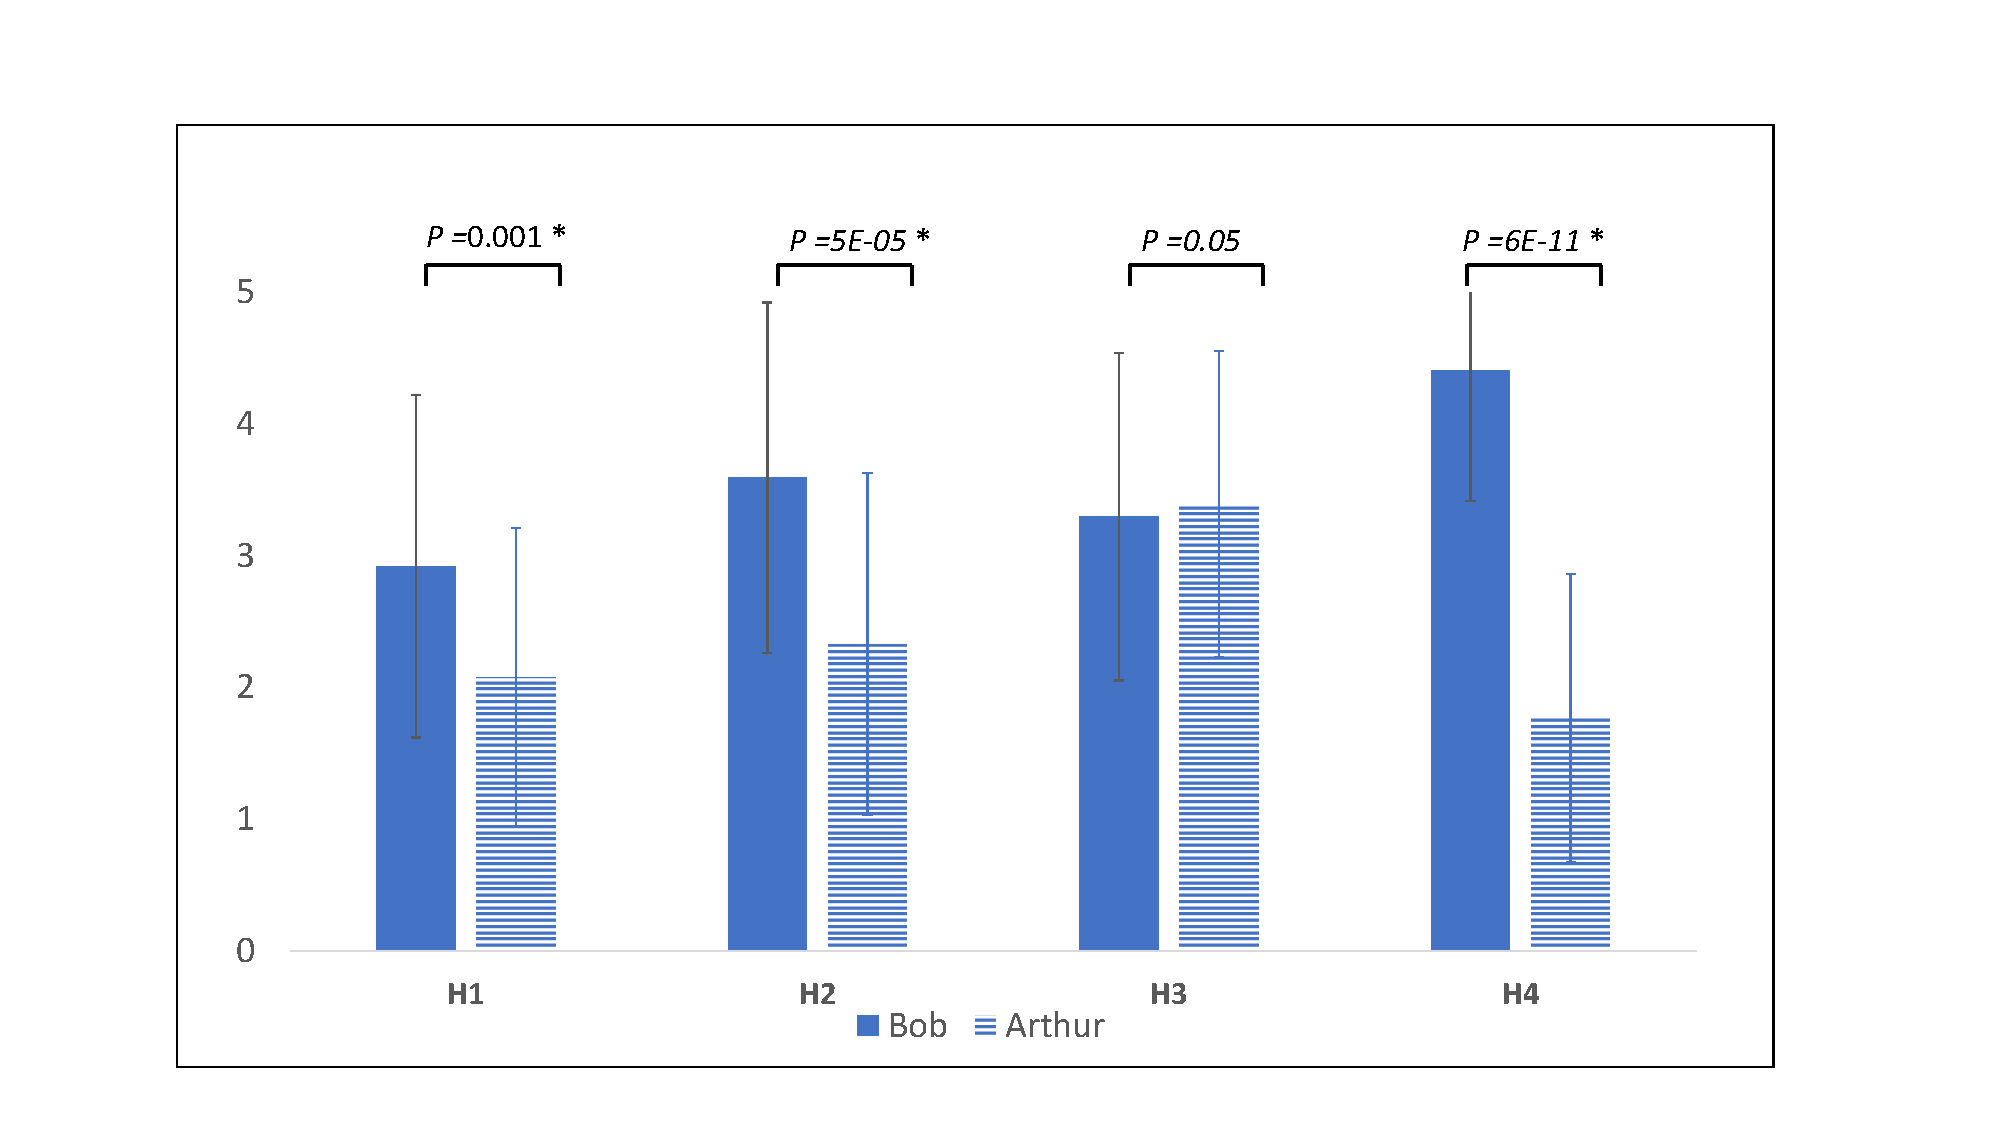
\includegraphics[width=0.5\textwidth,height=0.3\textheight]{graphs/res.pdf}
					\caption{Résultats de notre analyse}
					\label{res}
				\end{figure}